\documentclass[11pt,a4paper]{article}
\usepackage[T1]{fontenc}
\usepackage[utf8]{inputenc}
\usepackage{lmodern}
\usepackage{textcomp}
\usepackage{amsmath}
\usepackage[protrusion=true,expansion=true]{microtype}
\usepackage[a4paper,margin=2.4cm]{geometry}
\usepackage{setspace}
\usepackage[switch,modulo]{lineno}
\usepackage{graphicx}
\usepackage{float}
\usepackage{booktabs}
\usepackage{array}
\usepackage{tabularx}
\usepackage[table]{xcolor}
\usepackage[font=small,labelfont={bf,sf},skip=6pt]{caption}
\usepackage{subcaption}
\usepackage{enumitem}
\usepackage{fancyhdr}
\usepackage[explicit]{titlesec}
\usepackage[most]{tcolorbox}
\usepackage{needspace}
\usepackage{tikz}
\usetikzlibrary{positioning,arrows.meta,fit,backgrounds,calc}
\usepackage[style=vancouver,backend=biber,sorting=none,autocite=superscript,maxbibnames=6,minbibnames=6,useprefix=true]{biblatex}
\DeclareDelimFormat{finalnamedelim}{\addcomma\space}
\addbibresource{references.bib}
\usepackage{xurl}
\usepackage[hidelinks]{hyperref}

\definecolor{strap}{HTML}{2A78D6}
\definecolor{watch}{HTML}{EB6834}
\definecolor{ink}{HTML}{0B0B0B}
\definecolor{inksoft}{HTML}{52514E}
\definecolor{rule}{HTML}{C3C2B7}
\definecolor{wash}{HTML}{F0EFEC}
\definecolor{link}{HTML}{1C5CAB}
\definecolor{todo}{HTML}{B5470F}
\hypersetup{colorlinks=true,linkcolor=link,urlcolor=link,citecolor=link,
  pdftitle={Analytic choices can rival device error in real-world comparisons of wearable nocturnal heart rate variability}}

\newcommand{\todo}[1]{\textcolor{todo}{\textsf{[#1]}}}
% Generated by paper/build.py -- do not edit.
\newcommand{\benchAdjacentTen}{7.0}
\newcommand{\benchDeleteMax}{96}
\newcommand{\benchDeleteMin}{11}
\newcommand{\benchDeleteTen}{21.5}
\newcommand{\benchDeleteThirty}{62}
\newcommand{\benchInterpTen}{4.2}
\newcommand{\benchKubiosMax}{298}
\newcommand{\benchKubiosMin}{38}
\newcommand{\benchKubiosTen}{64.7}
\newcommand{\benchKubiosThirty}{132}
\newcommand{\benchLenientThirty}{5.0}
\newcommand{\benchLenientTwenty}{3.0}
\newcommand{\benchLenientYieldThirty}{86}
\newcommand{\benchLenientYieldTwenty}{100}
\newcommand{\benchNoneIso}{149}
\newcommand{\benchProposedTen}{1.9}
\newcommand{\benchProposedYieldThirty}{6}
\newcommand{\benchProposedYieldTwenty}{20}
\newcommand{\cleanSyntheticBias}{\textminus{}1.4}
\newcommand{\clockDeficitMin}{42.2}
\newcommand{\clockSpread}{9.7}
\newcommand{\correctedPct}{3.0}
\newcommand{\deviceAlsoFlagPct}{99}
\newcommand{\deviceCoveragePct}{8}
\newcommand{\deviceFlagged}{894}
\newcommand{\diffHOne}{+1.7}
\newcommand{\diffHThree}{\textminus{}8.0}
\newcommand{\diffHTwo}{+1.6}
\newcommand{\digMeanErrMean}{+0.01}
\newcommand{\digMeanErrNinetyFive}{1.72}
\newcommand{\digMeanErrSD}{0.87}
\newcommand{\digPrecision}{89}
\newcommand{\digRecall}{96}
\newcommand{\digTimeMedian}{0.33}
\newcommand{\digValueMedian}{0.19}
\newcommand{\digValueNinetyFive}{1.03}
\newcommand{\epochCCC}{0.39}
\newcommand{\epochRatioHigh}{1.60}
\newcommand{\epochRatioLow}{0.64}
\newcommand{\lagBest}{+20}
\newcommand{\lagBestR}{0.86}
\newcommand{\lagZeroR}{0.44}
\newcommand{\maskedMin}{147}
\newcommand{\maskedPct}{37}
\newcommand{\maxRRs}{3.03}
\newcommand{\mitAllEctopic}{34}
\newcommand{\mitAllErrProposed}{1.0}
\newcommand{\mitAllErrUncleaned}{130}
\newcommand{\mitAllFalseFlag}{1.4}
\newcommand{\mitAllSensitivity}{100.0}
\newcommand{\mitEctopic}{34}
\newcommand{\mitFalseFlag}{1.4}
\newcommand{\mitProposed}{27.8}
\newcommand{\mitRecords}{1}
\newcommand{\mitRef}{27.5}
\newcommand{\mitSensitivity}{100}
\newcommand{\mitUncleaned}{63.2}
\newcommand{\nCharts}{200}
\newcommand{\nDigReadings}{6{,}590}
\newcommand{\nHOne}{11}
\newcommand{\nHThree}{12}
\newcommand{\nHTwo}{7}
\newcommand{\nInvalidHOne}{31}
\newcommand{\nNoiseEpisodes}{573}
\newcommand{\nPoints}{42}
\newcommand{\nRR}{23{,}816}
\newcommand{\nReadings}{42}
\newcommand{\nRealSegments}{5}
\newcommand{\nSpecs}{36}
\newcommand{\nSpecsMain}{24}
\newcommand{\nValidHOne}{11}
\newcommand{\nightlySE}{1.8}
\newcommand{\noiseMedianS}{6.4}
\newcommand{\noiseNinetyS}{22}
\newcommand{\normalHalfWidth}{6}
\newcommand{\normalHigh}{68}
\newcommand{\normalLow}{56}
\newcommand{\normalWidth}{12}
\newcommand{\pitAdjacent}{\textminus{}20.0}
\newcommand{\pitAllRange}{253}
\newcommand{\pitDefMax}{+6.5}
\newcommand{\pitDefMin}{\textminus{}20.0}
\newcommand{\pitDefRange}{26.4}
\newcommand{\pitDelete}{\textminus{}43.7}
\newcommand{\pitInterp}{\textminus{}9.3}
\newcommand{\pitKubios}{\textminus{}161.7}
\newcommand{\pitNone}{\textminus{}250.9}
\newcommand{\pitUnmatched}{\textminus{}9.5}
\newcommand{\polylineRmse}{0.60}
\newcommand{\pxPerMs}{1.517}
\newcommand{\qualityGap}{15.6}
\newcommand{\rHOne}{0.44}
\newcommand{\rHThree}{0.29}
\newcommand{\rHTwo}{0.90}
\newcommand{\readingGaps}{2}
\newcommand{\readingSpacing}{10.1}
\newcommand{\realMinutes}{40}
\newcommand{\rhrFive}{45.2}
\newcommand{\rhrMean}{51.2}
\newcommand{\rhrOneMin}{44.3}
\newcommand{\rhrPFive}{45.5}
\newcommand{\rhrSpread}{6.9}
\newcommand{\rhrThirty}{46.6}
\newcommand{\rrDuration}{6~h~39~min}
\newcommand{\sessionDuration}{7~h~21~min}
\newcommand{\specAllMax}{+6.5}
\newcommand{\specAllMin}{\textminus{}12.5}
\newcommand{\specLenientMedian}{\textminus{}8.0}
\newcommand{\specMax}{+6.5}
\newcommand{\specMedian}{\textminus{}0.4}
\newcommand{\specMin}{\textminus{}8.0}
\newcommand{\strapFiveN}{77}
\newcommand{\strapFiveRMSSD}{57.5}
\newcommand{\strapFiveValid}{21}
\newcommand{\strapNone}{299}
\newcommand{\strapSD}{8.9}
\newcommand{\swAdjacentLowMax}{8.5}
\newcommand{\swAdjacentLowMin}{2.3}
\newcommand{\swInterpLowMax}{5.3}
\newcommand{\swInterpLowMin}{3.3}
\newcommand{\swInterpTwenty}{7.1}
\newcommand{\swNTwenty}{7}
\newcommand{\swProposedLowMax}{1.9}
\newcommand{\swProposedLowMin}{1.1}
\newcommand{\swProposedMax}{6.8}
\newcommand{\swProposedMin}{1.1}
\newcommand{\swProposedTwenty}{6.8}
\newcommand{\usableSleepPct}{64}
\newcommand{\watchDigitized}{47.98}
\newcommand{\watchExcessSD}{11.9}
\newcommand{\watchMatchedInvalid}{43.9}
\newcommand{\watchMatchedValid}{59.5}
\newcommand{\watchReported}{48}
\newcommand{\watchSD}{14.9}
\newcommand{\wordsAbstract}{299}
\newcommand{\wordsMain}{3{,}448}


\setstretch{1.25}
\setlength{\parskip}{3pt}
\setlist{nosep,leftmargin=1.4em,topsep=2pt}
\renewcommand{\arraystretch}{1.15}
\newcolumntype{Y}{>{\raggedright\arraybackslash}X}
\titleformat{\section}{\sffamily\Large\bfseries\color{ink}}{\thesection}{0.6em}{#1}
\titleformat{name=\section,numberless}{\sffamily\Large\bfseries\color{ink}}{}{0em}{#1}
\titleformat{\subsection}{\sffamily\large\bfseries\color{ink}}{\thesubsection}{0.6em}{#1}
\titleformat{name=\subsection,numberless}{\sffamily\large\bfseries\color{ink}}{}{0em}{#1}
\titlespacing*{\section}{0pt}{12pt}{3pt}
\titlespacing*{\subsection}{0pt}{8pt}{2pt}
\pagestyle{fancy}
\fancyhf{}
\renewcommand{\headrulewidth}{0.4pt}
\fancyhead[L]{\sffamily\small\color{inksoft}Analytic choices in wearable HRV comparisons}
\fancyhead[R]{\sffamily\small\color{inksoft}\thepage}
\newtcolorbox{keybox}[1]{enhanced,breakable,colback=wash,colframe=rule,boxrule=0.5pt,arc=2pt,
  left=8pt,right=8pt,top=6pt,bottom=6pt,fonttitle=\sffamily\bfseries,coltitle=ink,colbacktitle=wash,title={#1}}

\begin{document}
\thispagestyle{plain}
\begin{flushleft}
{\sffamily\bfseries\LARGE Analytic choices can rival device error in real-world comparisons of wearable nocturnal heart rate variability: a methods study with benchmark validation and a single-case illustration\par}
\vspace{10pt}
{\large \todo{Author names}\par}
\vspace{4pt}
{\small \todo{Affiliations}\par
\todo{Corresponding author: name, address, e-mail}\par
\vspace{4pt}
Running title: Analytic choices in wearable HRV comparisons\par
Article type: Methods / research article (exploratory) \quad
Word count (approximate): main text \wordsMain{}; abstract \wordsAbstract{}\par
Keywords: heart rate variability; wearable devices; RMSSD; artefact correction; method comparison; multiverse analysis; reproducibility\par}
\end{flushleft}

\section*{Abstract}
\textbf{Background.} Users and researchers increasingly check wearable nocturnal heart rate variability (HRV), usually the root mean square of successive differences (RMSSD), against consumer electrocardiographic chest straps. Real-world comparisons face three obstacles: artefact-dense reference RR series, wearable outputs available only as app charts, and unsynchronised device clocks. Their effect on the apparent wearable error is unknown.

\textbf{Methods.} We developed an open-source framework comprising time-preserving, classification-based artefact handling that masks noise bursts and uses only successive differences between adjacent usable beats; validated digitisation of app charts; explicit clock-deficit hypotheses without fitted offsets; and coverage-matched night-level comparison with a specification-curve (multiverse) analysis. We benchmarked artefact handling against five common approaches on real and synthetic NN series corrupted with isolated artefacts and contact noise covering 0--30\% of recording time, validated the digitiser on \nCharts{} synthetic charts with known readings, and illustrated the framework on one night of one adult (chest strap versus COROS watch).

\textbf{Results.} With 10\% of time contaminated, median absolute RMSSD error was \benchDeleteTen\% for deleting filtered beats, \benchKubiosTen\% for an open-source Kubios-type correction, \benchInterpTen\% for interpolation and \benchProposedTen\% for the proposed method, which declined to estimate windows with insufficient usable data (yield \benchProposedYieldTwenty\% at 20\% contamination). The digitiser recovered \digRecall\% of readings (median error \digValueMedian{}~ms). In the illustrative night, the apparent watch-minus-strap difference in nightly RMSSD was \pitNone{}~ms without cleaning; across defensible analyses it ranged from \pitDefMin{} to \pitDefMax{}~ms, a span wider than the watch's \normalWidth-ms personal normal range. Watch readings from strap-usable periods averaged \qualityGap{}~ms higher than the remaining readings.

\textbf{Conclusions.} In real-world comparisons, analytic choices can produce apparent wearable errors as large as the ranges used to interpret nightly HRV. Comparisons should pre-specify artefact handling, coverage matching and clock reconciliation, and report all defensible analyses. Definitive validation requires multi-participant, multi-night studies against electrocardiography.

\begin{keybox}{Key messages}
\textbf{What is already known.} Consumer wearables report nocturnal RMSSD, and laboratory studies against electrocardiography suggest nightly averages can be accurate for some devices. Editing of RR intervals is known to affect HRV.\\[3pt]
\textbf{What this study adds.} Real-world comparisons against a consumer chest strap involve three analytic choices that are rarely reported: artefact handling, coverage matching and clock reconciliation. In benchmarks with known ground truth, common artefact handling inflated RMSSD error by an order of magnitude under contact noise. In an illustrative night, defensible analyses alone moved the apparent wearable error by more than the wearable's own normal range.\\[3pt]
\textbf{How this might affect research and practice.} Wearable--reference comparisons should report a minimum set of analytic items (Table~\ref{tab:reporting}) and a multiverse of defensible analyses before attributing differences to the device.
\end{keybox}

\newpage
\linenumbers
\section{Introduction}
Consumer wearables now record physiological signals continuously, and the resulting data are entering medicine: resting heart rate and sleep from fitness trackers improved real-time surveillance of influenza-like illness at population level,\autocite{radin2020} and smartwatch data identified many COVID-19 infections before symptom onset.\autocite{mishra2020} Many devices also report nocturnal heart rate variability (HRV), typically the root mean square of successive differences (RMSSD), a time-domain index that reflects predominantly vagal modulation.\autocite{taskforce1996,shaffer2017} Validation studies against electrocardiography (ECG) suggest that nightly averages of RMSSD from some devices agree well with ECG, whereas agreement over short windows is weaker,\autocite{stone2021,cao2022} and expert recommendations now specify how such validations should be designed and reported.\autocite{muhlen2021} Optical devices measure pulse rate variability, which is not interchangeable with ECG-derived HRV.\autocite{schafer2013}

Outside the laboratory, people increasingly check a wearable against a consumer ECG chest strap, which can deliver RR intervals of high quality under good conditions.\autocite{gilgen2019} Such real-world comparisons face three practical obstacles. First, the reference RR series is often contaminated by contact artefacts, and the common editing choices---deleting, interpolating or correcting suspect beats---affect HRV differently.\autocite{peltola2012,clifford2005} Correction algorithms such as that of Lipponen and Tarvainen were designed for isolated ectopic, missed and extra beats.\autocite{lipponen2019} Second, wearable outputs are frequently available only as app summaries or charts, not as data. Third, the two devices' clocks are not synchronised, and a reference that reconstructs time from summed RR intervals silently loses time whenever beats are not recorded. Each obstacle forces analytic choices. Flexibility in such choices can change conclusions,\autocite{steegen2016,simonsohn2020} yet how far these choices alone can move an apparent wearable error has not, to our knowledge, been quantified.

We therefore (i) developed a transparent framework for real-world wearable--reference comparisons of nocturnal HRV; (ii) evaluated its artefact handling against common alternatives on data with known ground truth, and its chart digitisation on charts with known values; and (iii) illustrated, on one night of one person, how much each analytic choice changes the apparent wearable--reference difference. The night is used as an illustration, not as a validation of the wearable.

\section{Methods}
\subsection{Overview}
The framework (Figure~\ref{fig:framework}) processes three inputs: the reference RR export, the wearable's app chart and the two device clocks. Its output is a coverage-matched night-level comparison reported across all defensible analytic choices. We followed the Guidelines for Reporting Reliability and Agreement Studies where applicable,\autocite{kottner2011} and report HRV methods following GRAPH.\autocite{quintana2016}

\begin{figure}[t]
\centering
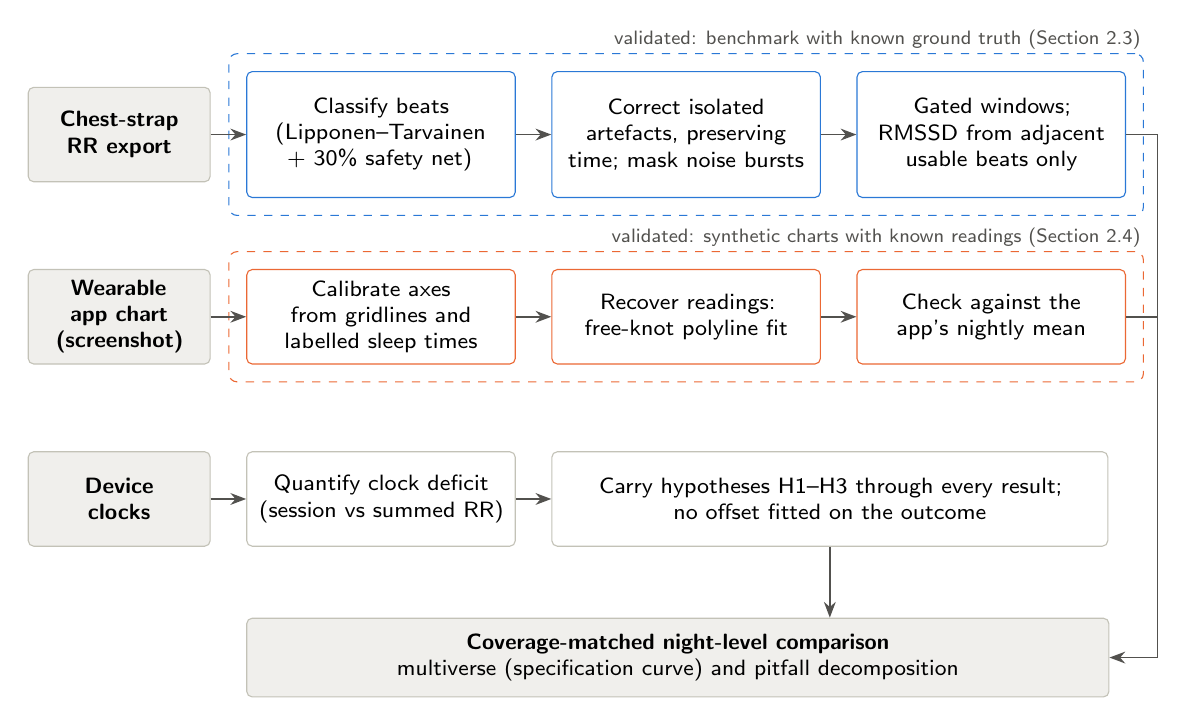
\begin{tikzpicture}[font=\sffamily\footnotesize, node distance=11mm and 4.5mm,
  box/.style={draw=rule, rounded corners=2pt, fill=white, text width=32mm, align=center, minimum height=12mm, inner sep=3pt, execute at begin node={\hyphenpenalty=10000\exhyphenpenalty=10000}},
  inp/.style={box, fill=wash, text width=21mm, font=\sffamily\footnotesize\bfseries},
  arr/.style={-{Stealth[length=2mm]}, draw=inksoft, line width=0.6pt},
  grp/.style={draw, dashed, rounded corners=3pt, inner sep=2.2mm},
  glabel/.style={font=\sffamily\scriptsize, text=inksoft, anchor=south east, inner sep=1pt}]
  \node[inp] (s0) {Chest-strap\\RR export};
  \node[box, right=of s0, draw=strap, minimum height=16mm] (s1) {Classify beats (Lipponen--Tarvainen + 30\% safety net)};
  \node[box, right=of s1, draw=strap, minimum height=16mm] (s2) {Correct isolated artefacts, preserving time; mask noise bursts};
  \node[box, right=of s2, draw=strap, minimum height=16mm] (s3) {Gated windows; RMSSD from adjacent usable beats only};
  \node[inp, below=of s0] (w0) {Wearable app chart (screenshot)};
  \node[box, right=of w0, draw=watch] (w1) {Calibrate axes from gridlines and labelled sleep times};
  \node[box, right=of w1, draw=watch] (w2) {Recover readings: free-knot polyline fit};
  \node[box, right=of w2, draw=watch] (w3) {Check against the app's nightly mean};
  \node[inp, below=of w0] (c0) {Device\\clocks};
  \node[box, right=of c0] (c1) {Quantify clock deficit (session vs summed RR)};
  \node[box, right=of c1, text width=68.5mm] (c2) {Carry hypotheses H1--H3 through every result;\\no offset fitted on the outcome};
  \path let \p1 = (c1.south west), \p2 = (c2.south east) in
    node[box, fill=wash, anchor=north west, minimum width={\x2-\x1}, minimum height=10mm, text width=, align=center] (m) at (\x1, \y1-9mm)
    {\textbf{Coverage-matched night-level comparison}\\multiverse (specification curve) and pitfall decomposition};
  \foreach \a/\b in {s0/s1,s1/s2,s2/s3,w0/w1,w1/w2,w2/w3,c0/c1,c1/c2} \draw[arr] (\a) -- (\b);
  \draw[arr] (s3.east) -- ++(4mm,0) |- (m.east);
  \draw[draw=inksoft, line width=0.6pt] (w3.east) -- ++(4mm,0);
  \draw[arr] (c2.south) -- (c2.south |- m.north);
  \begin{scope}[on background layer]
    \node[grp, draw=strap, fit=(s1)(s3)] (g1) {};
    \node[grp, draw=watch, fit=(w1)(w3)] (g2) {};
  \end{scope}
  \node[glabel] at (g1.north east) {validated: benchmark with known ground truth (Section 2.3)};
  \node[glabel] at (g2.north east) {validated: synthetic charts with known readings (Section 2.4)};
\end{tikzpicture}
\caption{Framework for real-world comparison of wearable nocturnal HRV with a chest-strap reference. Boxes are processing steps; dashed outlines mark the steps validated in this paper.}
\label{fig:framework}
\end{figure}

\subsection{Artefact handling in the reference RR series}
Intervals outside 400--2000~ms (30--150 beats per minute, appropriate for sleep) were flagged. Each interval was then classified as normal, ectopic, missed, extra or long/short by the algorithm of Lipponen and Tarvainen, which uses time-varying thresholds (5.2 times the quartile deviation over 91 beats) on successive differences and on deviations from an 11-beat median.\autocite{lipponen2019} We made three changes for contact-noise-dense data. First, thresholds were computed only from beats not already flagged, because noise otherwise widens them until obvious artefacts pass. Second, as a fixed safety net, any interval deviating more than 30\% from a 45-beat median was flagged. Third, where at least 3 of any 10 consecutive intervals were flagged, the run (with 2 intervals either side) was \emph{masked} rather than corrected, because correcting a run of noise would fabricate beats. Masked intervals keep their duration, so the time axis stays continuous and every analysis window knows how much of its time is unusable.

Isolated artefacts were corrected in the beat-time domain so that total elapsed time is preserved exactly: an extra detection was merged with the neighbour whose sum best matched the local median; a missed beat was split into equal intervals; an ectopic or long/short interval was corrected by moving the R-peak shared by a pair of intervals to their midpoint. Detection was repeated on the corrected series, and any interval still flagged was masked. RMSSD was computed only from successive differences between two adjacent usable intervals, so no difference spans a gap. Spectral power, when reported, used the Lomb--Scargle periodogram on the unevenly spaced usable beats,\autocite{laguna1998,clifford2005} so masked gaps never needed interpolation. An analysis window was retained only if at least 80\% of its duration was usable NN time and at most 5\% of its beats had been corrected (default gate); a lenient gate (60\%, 10\%) was used in sensitivity analyses.

\subsection{Benchmark validation of artefact handling}
\textit{Ground truth.} We used two sources of artefact-free NN series. The real source comprised the \nRealSegments{} stretches of the illustrative night (\realMinutes{}~min in total) that were clean by two independent criteria: no interval flagged by the proposed method and no successive change above 20\%. The synthetic source comprised 20 ten-minute series combining respiratory sinus arrhythmia (amplitude 10--60~ms at 0.20--0.30~Hz), a 0.1-Hz oscillation (5--30~ms) and white noise (5--20~ms), at mean RR intervals of 850--1300~ms.

\textit{Corruption.} Each series was corrupted with isolated artefacts at 1\% of beats (ectopic beats as a 65\% coupling interval with compensatory pause, missed beats and extra detections) and with contact-noise episodes covering 0, 5, 10, 20 or 30\% of the recording time. Every episode replaced a stretch of beats of exactly the same total duration, so wall-clock windows of the corrupted series align with those of the clean series. Empirical episodes were \nNoiseEpisodes{} runs of contact noise cut from the illustrative night with a rule independent of the proposed method (intervals deviating more than 30\% from a 91-beat rolling median, merged and padded; median duration \noiseMedianS{}~s, 90th percentile \noiseNinetyS{}~s). Parametric episodes were random detections of 250--1500~ms with the same duration distribution. Each condition was repeated with 5 (real) or 3 (synthetic) random seeds.

\textit{Comparators.} We compared: no cleaning; a 20\% filter (relative to the last accepted interval, with the same 400--2000~ms range and a reset after 5 consecutive rejections), followed by deletion with differences taken across the gaps, by deletion with differences restricted to originally adjacent beats, or by linear interpolation; the Lipponen--Tarvainen correction as implemented in NeuroKit2 0.2.13 (iterative, without any exclusion rule);\autocite{makowski2021,lipponen2019} and the proposed method with the default and the lenient gate.

\textit{Outcomes.} For each 5-min window we compared the estimated RMSSD with the RMSSD of the clean series in the same window, and summarised the median absolute percentage error and the proportion of windows for which a method produced an estimate. Because the proposed method declines to estimate poor windows, we also compared all methods on exactly the windows it retained. \ifnum\mitRecords>1 As a check with real ectopy, we applied the method to the \mitRecords{} records of the MIT-BIH Arrhythmia Database without pacing, atrial fibrillation or flutter, whose beats are expert-annotated,\autocite{moody2001,goldberger2000} and compared RMSSD with the reference computed from adjacent normal-to-normal intervals.\else As a check with real ectopy, we applied the method to MIT-BIH Arrhythmia Database record~100, whose beats are expert-annotated,\autocite{moody2001,goldberger2000} and compared RMSSD with the reference computed from adjacent normal-to-normal intervals. Validation on the full MIT-BIH Arrhythmia Database is implemented but could not be run in our computing environment, which did not permit access to PhysioNet; it is reported as pending.\fi

\subsection{Recovering wearable readings from app charts}
The app chart was calibrated from its own rendering: horizontal gridlines labelled 0, 50, 100 and 150~ms were detected and fitted linearly (\pxPerMs{} pixels per millisecond), and the baseline was mapped to the labelled sleep onset and wake times. The line was traced as the per-column centroid of line-coloured pixels. The readings---the vertices of the polyline---were recovered by seeding knots where the local slope changes, estimating knot values by least squares on a piecewise-linear basis (so that a vertex's value comes from the straight segments on either side rather than from the rounded corner of the anti-aliased line), refining knot positions locally and adding knots wherever the fit missed the drawn line. The digitised nightly mean was checked against the app's reported nightly mean.

To validate the digitiser, we removed the line from the real screenshot and drew \nCharts{} synthetic nights into the app's own screen (gridlines, labels and icons unchanged). Readings were placed about every 10~minutes with occasional skipped readings and values from an autoregressive process (12--140~ms), drawn in the app's line colour and width with anti-aliasing. Recovered readings were matched to true readings within $\pm$5~min.

\subsection{Reconciling device clocks}
Chest straps of this kind timestamp beats as the session start plus the cumulative sum of RR intervals, so any period without recorded beats (for example, during contact loss) disappears from the reference clock. We quantified the deficit as the session duration minus the summed RR intervals and carried three hypotheses through every analysis: H1, the reference clock taken as recorded (the beat stream ended early); H2, the missing time spread uniformly over the night; and H3, the missing time located inside the masked noise episodes in proportion to their duration. We did not fit a time offset, because an offset chosen to maximise agreement would inflate the agreement subsequently reported. A lag scan is shown only as a diagnostic.

\subsection{Agreement analysis}
The principal estimand was the \emph{coverage-matched night-level difference}: the mean of the wearable readings whose matched reference window passed the gate, minus the mean RMSSD of those reference windows. The reference window was the 10~minutes ending at each reading. Epoch-level agreement was summarised descriptively by Bland--Altman limits of agreement on the logarithmic scale, back-transformed to ratios,\autocite{bland1986,bland1999} and Lin's concordance correlation coefficient.\autocite{lin1989} We report no $p$-values for the illustrative night, because epochs from one night are few and autocorrelated.\autocite{bland2007} The multiverse comprised every combination of clock hypothesis (3), gate (strict ${\geq}90\%$ usable and ${\leq}2\%$ corrected, default, lenient), window convention (ending at or centred on the reading) and window length (10 or 5~min), giving \nSpecs{} specifications, displayed as a specification curve.\autocite{steegen2016,simonsohn2020} In a pitfall decomposition we compared the wearable's reported nightly mean with the reference's whole-night mean of 5-min RMSSD under each artefact-handling method, and then with the coverage-matched estimate under each clock hypothesis. We classed as defensible the artefact-handling methods whose median benchmark error was below 10\% at 10\% contamination (adjacency-restricted deletion, interpolation and the proposed method, with or without coverage matching) and every specification of the multiverse; the others were classed as naive.

\subsection{Illustrative night}
One adult \todo{age, sex, height, body mass and health status} wore a consumer ECG chest strap transmitting RR intervals (firmware 1.7.9; \todo{manufacturer and model}) and a COROS watch \todo{model} during one night (17 April 2026). The strap session ran for \sessionDuration{} from 02:19:50, and its RR export contained \nRR{} intervals. The watch, which measures overnight HRV as RMSSD at about 10-minute intervals during sleep and reports the night's average,\autocite{coros_hrv} detected sleep from 02:29 to 09:37 and reported a nightly mean of \watchReported{}~ms with a personal normal range of \normalLow--\normalHigh{}~ms. Its readings were available only as an app screenshot. The analysis was developed on these data; all choices are therefore exploratory and are reported as a multiverse.

\subsection{Software, data and reproducibility}
All analyses used an open-source Python package (hrvcompare) with NumPy, SciPy, pandas, NeuroKit2 and wfdb. A single build script runs every analysis and writes every number, table and figure in this manuscript; random seeds are deterministic. \todo{Repository URL and archived version (DOI)}.

\section{Results}
\subsection{Benchmark of artefact handling}
Isolated artefacts at 1\% of beats inflated uncleaned RMSSD by a median of \benchNoneIso\% (Table~\ref{tab:benchmark}). All filtering and correction methods handled isolated artefacts well, but contact noise separated them sharply (Figure~\ref{fig:benchmark}). With 10\% of time contaminated, median absolute error was \benchDeleteTen\% for deletion with differences taken across gaps, \benchAdjacentTen\% when differences were restricted to adjacent beats, \benchInterpTen\% for interpolation, \benchKubiosTen\% for the Kubios-type correction and \benchProposedTen\% for the proposed method. Across the contaminated conditions in Table~\ref{tab:benchmark}, errors ranged from \benchDeleteMin\% to \benchDeleteMax\% for deletion and from \benchKubiosMin\% to \benchKubiosMax\% for the Kubios-type correction, an algorithm designed for isolated ectopic, missed and extra beats rather than runs of noise.

The proposed method's accuracy came with fewer estimates: with the default gate it estimated \benchProposedYieldTwenty\% of windows at 20\% contamination and \benchProposedYieldThirty\% at 30\%. With the lenient gate it retained \benchLenientYieldTwenty\% and \benchLenientYieldThirty\% of windows, with errors of \benchLenientTwenty\% and \benchLenientThirty\%. Its advantage was not only a selection effect: on exactly the windows it retained at 5--10\% contamination, its median error was \swProposedLowMin--\swProposedLowMax\%, against \swInterpLowMin--\swInterpLowMax\% for interpolation and \swAdjacentLowMin--\swAdjacentLowMax\% for adjacency-restricted deletion; at 20\% the advantage narrowed (\swProposedTwenty\% versus \swInterpTwenty\% for interpolation with real ground truth, from only \swNTwenty{} windows; Supplementary Table~S1). On clean synthetic data, false flags biased its RMSSD by \cleanSyntheticBias\%. \ifnum\mitRecords>1 Across the \mitRecords{} MIT-BIH records, \mitAllSensitivity\% of \mitAllEctopic{} annotated ectopic beats were flagged; the median absolute RMSSD error against the reference was \mitAllErrProposed\% (uncleaned \mitAllErrUncleaned\%), and a median of \mitAllFalseFlag\% of normal intervals away from ectopy were flagged.\else In MIT-BIH record~100, \mitSensitivity\% of the \mitEctopic{} annotated ectopic beats were flagged; RMSSD was \mitProposed{}~ms against a reference of \mitRef{}~ms (uncleaned \mitUncleaned{}~ms), and \mitFalseFlag\% of normal intervals away from ectopy were flagged.\fi

\begin{table}[t]
\centering\small
\caption{Median absolute error (\%) of 5-min RMSSD by method and proportion of recording time contaminated by contact noise; 1\% of beats also carried isolated ectopic, missed or extra beats. For the proposed method, the percentage of windows with an estimate is shown in parentheses (100\% for all other methods).}
\label{tab:benchmark}
\begin{tabular}{lrrrrr}
\toprule
Method & 0\% & 5\% & 10\% & 20\% & 30\% \\
\midrule
\multicolumn{6}{l}{\textit{Real ground truth, empirical strap noise}} \\
No cleaning & 148.8 & 272.1 & 333.4 & 473.8 & 514.3 \\
20\% filter, delete & 0.5 & 11.0 & 21.5 & 44.9 & 62.0 \\
20\% filter, delete, adjacent pairs only & 0.3 & 2.3 & 7.0 & 14.3 & 20.9 \\
20\% filter, interpolate & 0.9 & 3.3 & 4.2 & 8.5 & 11.7 \\
Kubios-type correction (NeuroKit2) & 3.4 & 39.6 & 64.7 & 119.2 & 131.7 \\
Proposed & 0.4 \textcolor{inksoft}{(100)} & 1.1 \textcolor{inksoft}{(100)} & 1.9 \textcolor{inksoft}{(97)} & 6.8 \textcolor{inksoft}{(20)} & 12.1 \textcolor{inksoft}{(6)} \\
Proposed, lenient gate & 0.4 \textcolor{inksoft}{(100)} & 1.1 \textcolor{inksoft}{(100)} & 1.8 \textcolor{inksoft}{(100)} & 3.0 \textcolor{inksoft}{(100)} & 5.0 \textcolor{inksoft}{(86)} \\
\midrule
\multicolumn{6}{l}{\textit{Synthetic ground truth, parametric noise}} \\
No cleaning & 176.5 & 342.2 & 433.1 & 561.3 & 649.4 \\
20\% filter, delete & 0.4 & 13.9 & 30.5 & 67.8 & 95.5 \\
20\% filter, delete, adjacent pairs only & 0.3 & 3.3 & 5.1 & 17.1 & 28.2 \\
20\% filter, interpolate & 0.9 & 3.7 & 4.6 & 13.0 & 20.0 \\
Kubios-type correction (NeuroKit2) & 2.9 & 37.5 & 73.1 & 178.8 & 298.2 \\
Proposed & 1.2 \textcolor{inksoft}{(91)} & 1.5 \textcolor{inksoft}{(86)} & 1.4 \textcolor{inksoft}{(63)} & 1.9 \textcolor{inksoft}{(5)} & 5.8 \textcolor{inksoft}{(2)} \\
Proposed, lenient gate & 1.5 \textcolor{inksoft}{(100)} & 1.7 \textcolor{inksoft}{(100)} & 2.0 \textcolor{inksoft}{(99)} & 2.2 \textcolor{inksoft}{(87)} & 2.3 \textcolor{inksoft}{(35)} \\
\bottomrule
\end{tabular}

\end{table}

\begin{figure}[t]
\centering
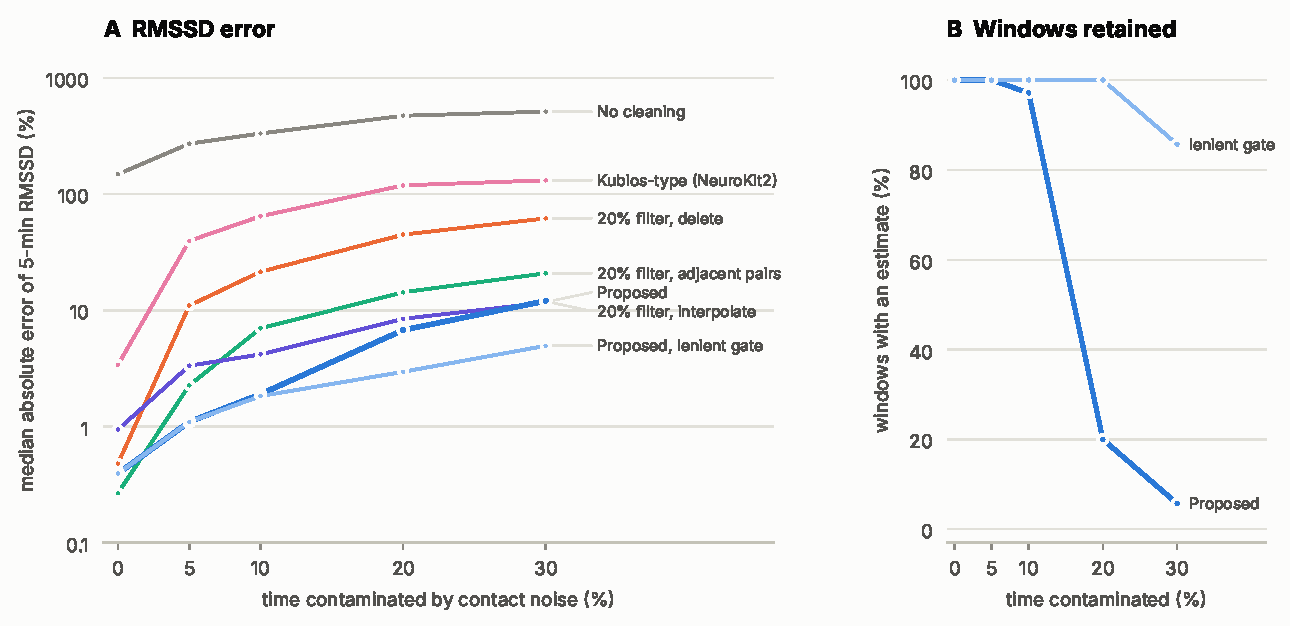
\includegraphics[width=\linewidth]{figures/fig2_benchmark.pdf}
\caption{Benchmark with real ground truth and empirical contact noise. (A) Median absolute error of 5-min RMSSD, logarithmic scale. (B) Proportion of windows for which the proposed method produced an estimate. All conditions are shown in Supplementary Figure~S1.}
\label{fig:benchmark}
\end{figure}

\subsection{Digitiser validation}
Across \nCharts{} synthetic nights, the digitiser recovered \digRecall\% of readings (precision \digPrecision\%), with a median absolute value error of \digValueMedian{}~ms (95th percentile \digValueNinetyFive{}~ms) and a median timing error of \digTimeMedian{}~min. The error of the digitised nightly mean averaged \digMeanErrMean{}~ms (SD \digMeanErrSD{}~ms; 95th percentile of absolute error \digMeanErrNinetyFive{}~ms; Supplementary Figure~S2). Spurious vertices lie on the drawn line and therefore change values little.

\subsection{Illustrative night}
\textit{Reference data quality.} Contact noise made \maskedPct\% of the recording (\maskedMin{}~min) unusable, and \correctedPct\% of usable beats were corrected (Figure~\ref{fig:night}a). The strap's own artefact flag marked \deviceFlagged{} beats; the framework flagged \deviceAlsoFlagPct\% of these, but they covered only \deviceCoveragePct\% of what the framework flagged. Of the sleep period covered by the strap, \usableSleepPct\% was usable.

\textit{Wearable data.} The digitiser recovered \nReadings{} readings at a median spacing of \readingSpacing{}~min with \readingGaps{} gaps longer than 15~min; their mean was \watchDigitized{}~ms against the app's \watchReported{}~ms (Figure~\ref{fig:night}b).

\textit{Clock.} The session lasted \sessionDuration, but the summed RR intervals covered only \rrDuration: \clockDeficitMin{}~min of wall-clock time contained no beats. No interval longer than \maxRRs{}~s occurred, so contact losses longer than that leave no trace. Under H1 the strap's final noise burst falls in the middle of sleep; under H2 and H3 it coincides with waking and the end of the session. The lag scan peaked at a shift of \lagBest{}~min ($r=\lagBestR$, against \lagZeroR{} unshifted; Supplementary Figure~S3), consistent with a reference clock running behind, but because it is selected on the outcome it was not used.

\textit{Coverage and selection.} Under H1, \nValidHOne{} of \nPoints{} watch readings had a reference window that passed the gate, mostly in the second half of the night. Watch readings in these windows averaged \watchMatchedValid{}~ms, against \watchMatchedInvalid{}~ms in the \nInvalidHOne{} others: the periods in which the reference was usable were systematically different from the rest of the night.

\textit{Apparent wearable error.} Compared with the watch's reported nightly mean, the uncleaned strap made the watch appear \pitNone{}~ms in error; Kubios-type correction, \pitKubios{}~ms; deletion, \pitDelete{}~ms; adjacency-restricted deletion, \pitAdjacent{}~ms; interpolation, \pitInterp{}~ms; and the proposed method without coverage matching, \pitUnmatched{}~ms (Figure~\ref{fig:pitfalls}). With coverage matching the difference was \diffHOne{}~ms under H1 ($n=\nHOne$ windows), \diffHTwo{}~ms under H2 ($n=\nHTwo$) and \diffHThree{}~ms under H3 ($n=\nHThree$): clock uncertainty alone moved it by \clockSpread{}~ms. Across the \nSpecsMain{} specifications with the strict or default gate, the night-level difference ranged from \specMin{} to \specMax{}~ms (median \specMedian{}~ms); with the lenient gate, whose windows contain more residual artefact, the median was \specLenientMedian{}~ms (Figure~\ref{fig:spec}). Across all defensible analyses the difference ranged from \pitDefMin{} to \pitDefMax{}~ms, a span of \pitDefRange{}~ms.

\textit{Single readings.} Individual watch readings scattered more than the reference (SD \watchSD{} versus \strapSD{}~ms in matched windows), implying about \watchExcessSD{}~ms of additional variation per reading; averaged over \nReadings{} readings, if independent, this shrinks to about \nightlySE{}~ms. Under H1, the 95\% limits of agreement for single readings were $\times$\epochRatioLow{} to $\times$\epochRatioHigh{} (concordance \epochCCC; Supplementary Figure~S4).

\textit{Resting heart rate.} Strap-derived resting heart rate ranged from \rhrOneMin{} to \rhrMean{}~bpm depending on its definition (lowest 1-min mean to mean over sleep; Supplementary Table~S6), a spread of \rhrSpread{}~bpm in the same night. The watch's value was not available.

\begin{figure}[p]
\centering
\begin{subfigure}{\linewidth}\centering
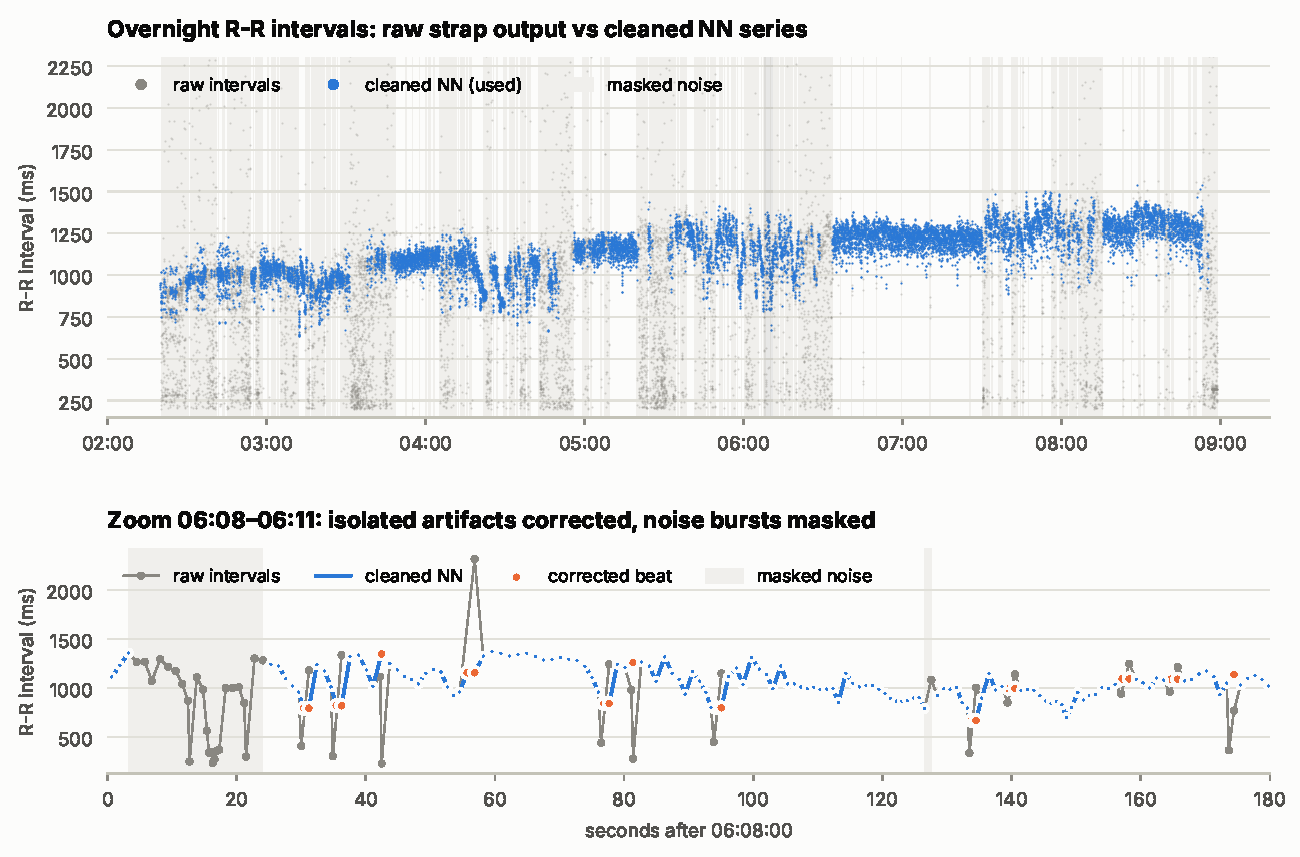
\includegraphics[width=0.92\linewidth]{figures/fig3a_tachogram.pdf}
\caption{Raw strap intervals and the cleaned NN series, with a 3-minute zoom.}
\end{subfigure}\\[6pt]
\begin{subfigure}{\linewidth}\centering
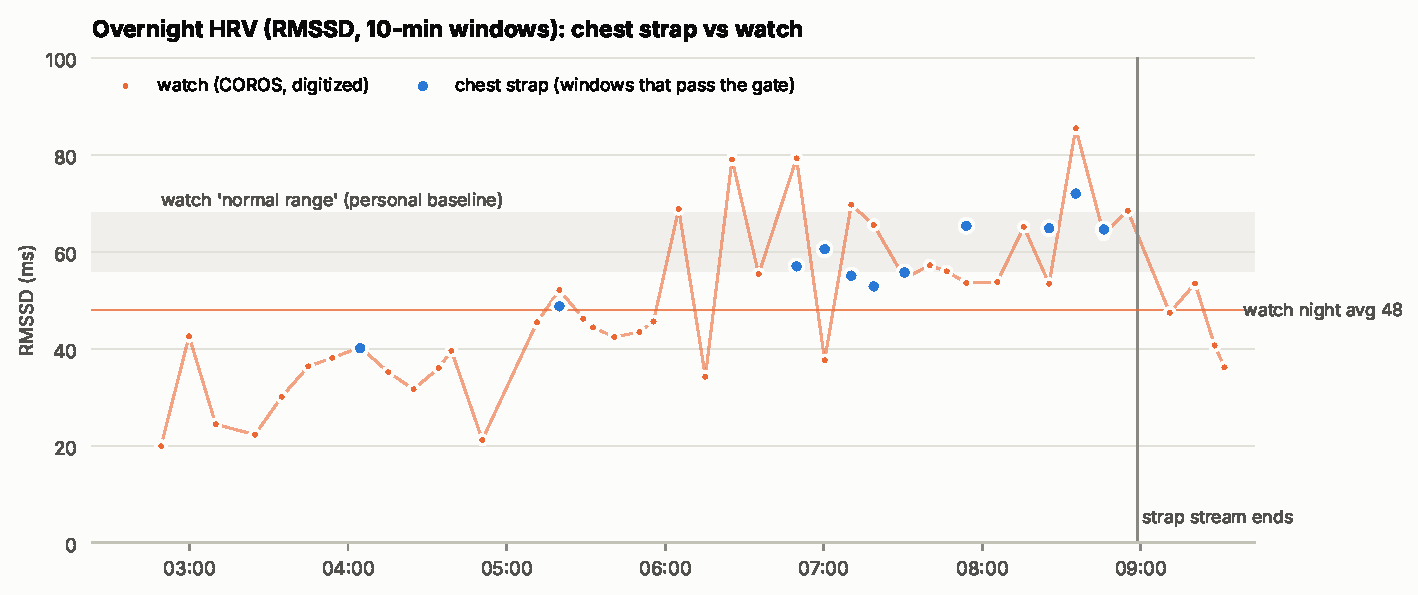
\includegraphics[width=0.92\linewidth]{figures/fig3b_rmssd_overnight.pdf}
\caption{Digitised watch readings and strap RMSSD in windows passing the gate (clock H1).}
\end{subfigure}
\caption{The illustrative night.}
\label{fig:night}
\end{figure}

\begin{figure}[t]
\centering
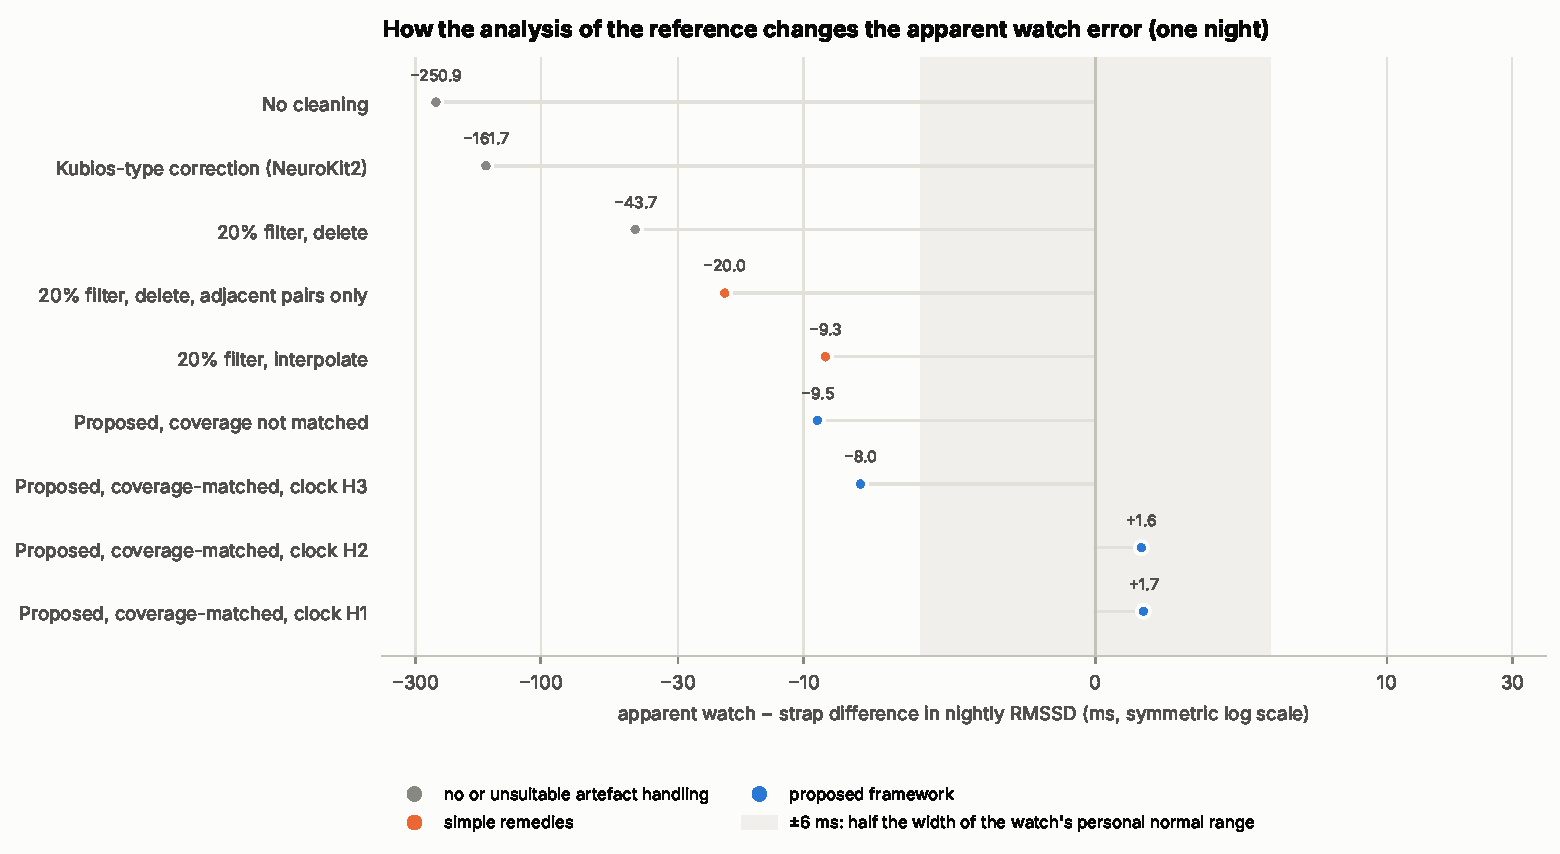
\includegraphics[width=\linewidth]{figures/fig4_pitfalls.pdf}
\caption{Pitfall decomposition for the illustrative night: the apparent watch-minus-strap difference in nightly RMSSD under successive analyses of the reference. The first six rows compare the watch's reported nightly mean with the strap's whole-night mean; the last three are coverage-matched under each clock hypothesis. Values are listed in Supplementary Table~S2.}
\label{fig:pitfalls}
\end{figure}

\begin{figure}[t]
\centering
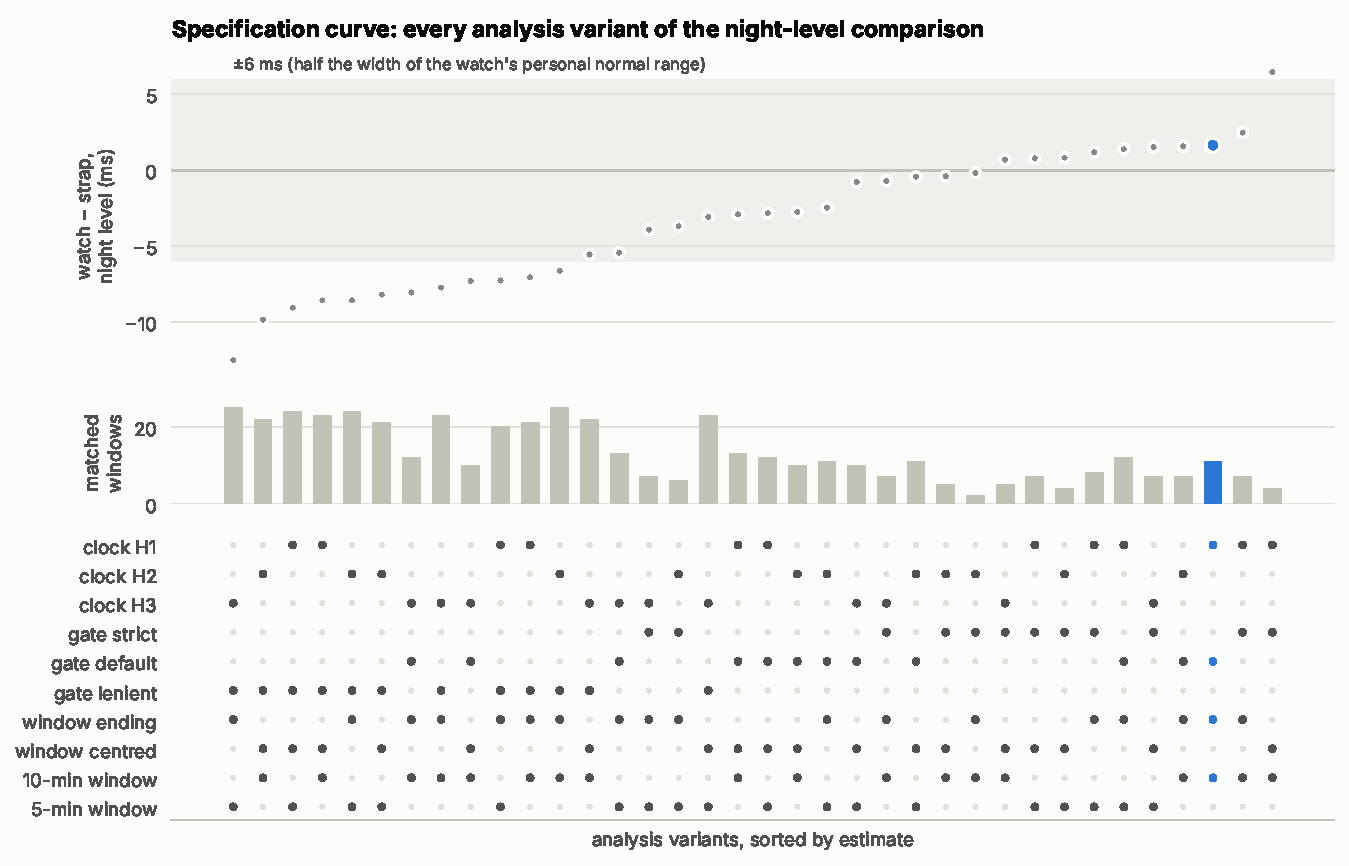
\includegraphics[width=\linewidth]{figures/fig5_specification_curve.pdf}
\caption{Specification curve of the coverage-matched night-level difference across all \nSpecs{} analysis variants. Blue marks the variant used in the other figures. The shaded band is $\pm$\normalHalfWidth{}~ms, half the width of the watch's personal normal range.}
\label{fig:spec}
\end{figure}

\section{Discussion}
\subsection{Principal findings}
Three analytic choices, rarely reported in wearable--reference comparisons, can each produce apparent wearable errors as large as those that comparisons seek to detect. First, artefact handling: under realistic contact noise, deleting filtered beats or applying a correction designed for isolated ectopy inflated RMSSD error by an order of magnitude, whereas restricting successive differences to adjacent beats---a one-line change---removed most of deletion's damage, and masking noise bursts with an explicit quality gate kept median errors at \swProposedMin--\swProposedMax\% on the windows it retained at 5--20\% contamination, at the cost of fewer estimates. Second, coverage: the periods in which a chest strap works well are not representative of the night, so comparing a wearable's whole-night summary with the reference's usable periods confounds device error with selection. Third, clock reconciliation: in the illustrative night, plausible assumptions about missing reference time alone moved the matched difference by \clockSpread{}~ms. Together, defensible analyses spanned \pitDefRange{}~ms, more than the \normalWidth-ms personal normal range the watch used to label the night as low.

\subsection{Comparison with previous work}
Laboratory and home studies against ECG have reported good agreement for nightly RMSSD from some wearables, with weaker agreement over short windows.\autocite{stone2021,cao2022} Our findings do not contradict these: they concern comparisons in which the reference itself is imperfect, and show that its processing can dominate the comparison. That editing strategies change HRV is well established,\autocite{peltola2012} and interpolation and resampling bias spectral estimates.\autocite{clifford2005} Our benchmark adds that correction algorithms designed for sparse ectopy\autocite{lipponen2019} fail when artefacts arrive in dense runs, and that masking such runs is preferable to correcting them. The wearable's additional per-reading variation is consistent with readings taken from short samples, for which RMSSD is valid on average but noisier.\autocite{munoz2015} The selection effect we observed is expected physiologically: HRV depends on sleep stage,\autocite{herzig2018} and chest-strap contact is plausibly most stable during undisturbed sleep. Finally, optical wearables measure pulse rate variability, which differs from ECG-derived HRV,\autocite{schafer2013} and inaccuracy of optical sensors differs between devices and activities;\autocite{bent2020} our framework treats the wearable output as a black box and does not resolve these sources.

\subsection{Implications}
Wearable--reference comparisons outside the laboratory should pre-specify, and report, how each of these choices was made. We propose a minimum set of items (Table~\ref{tab:reporting}) to complement existing recommendations for validation studies,\autocite{muhlen2021,kottner2011,quintana2016} and suggest that, where choices remain open, results be reported as a multiverse rather than as a single estimate.\autocite{steegen2016,simonsohn2020} For individual users and clinicians, a single-night difference of a few milliseconds between a wearable and a chest strap should not be read as device error without considering these analytic uncertainties.

\begin{table}[t]
\centering\small
\caption{Proposed minimum reporting items for real-world comparisons of wearable HRV with a reference.}
\label{tab:reporting}
\begin{tabularx}{\linewidth}{>{\raggedright\arraybackslash}p{0.27\linewidth}Y}
\toprule
\textbf{Domain} & \textbf{Item} \\
\midrule
Reference signal & Device, sensing principle (ECG or optical), RR resolution, availability of the raw signal \\
Artefact detection & Algorithm, thresholds and software version \\
Artefact handling & Per artefact type: corrected, masked or deleted; whether elapsed time is preserved \\
Successive differences & Whether differences may span removed beats \\
Windows and quality gate & Window length, coverage and correction thresholds, proportion of windows retained \\
Wearable output & Source (export, interface or screenshot); metric definition (window, pulse or heart rate variability) \\
Digitisation & Method and its validation, if outputs were read from images \\
Clock reconciliation & Anchors, drift and missing time; whether any offset was estimated from the outcome \\
Coverage matching & Which periods each device's summary covers \\
Estimand and statistics & Night-level or epoch-level; agreement statistics on a suitable scale; handling of repeated measures \\
Analytic flexibility & Pre-specification; multiverse or sensitivity analysis across defensible choices \\
Transparency & Data and code availability \\
\bottomrule
\end{tabularx}
\end{table}

\subsection{Strengths and limitations}
The framework is fully reproducible, preserves elapsed time by construction and is validated against known ground truth, and the multiverse makes analytic flexibility visible rather than hidden. The limitations are substantial. The illustration is one night of one person and supports no inference about the device; the reference is a consumer chest strap without access to the raw ECG, so artefacts could not be adjudicated visually. The real ground truth in the benchmark is short and was selected partly by the proposed method, and the empirical noise library comes from the same night and was cut with a 30\% deviation rule that resembles the method's own safety net, which may favour the method; the synthetic data rest on modelling assumptions. \ifnum\mitRecords>1 External validation covered ectopy in one annotated database; long clean NN series from other databases remain to be tested.\else External validation on an annotated database is implemented but pending.\fi The digitiser was validated in one app's visual style only. The Kubios-type comparator was an open-source implementation of the published algorithm applied to all artefacts; commercial software that handles noisy segments separately may perform differently. The wearable's algorithm is proprietary. The analysis was developed on the same night it illustrates; the multiverse mitigates but does not remove this. No sleep staging was available.

A definitive evaluation should enrol multiple participants over multiple nights with a criterion ECG (Holter or polysomnography), pre-register its analysis plan, size the study for the precision of the limits of agreement,\autocite{bland1986,lu2016} use methods for repeated measurements per person,\autocite{bland2007} and obtain wearable data through an export rather than screenshots.

\section{Conclusions}
In real-world comparisons of wearable nocturnal HRV with a chest strap, the handling of reference artefacts, the matching of coverage and the reconciliation of clocks can each change the apparent wearable error by as much as the ranges used to interpret it. These choices should be pre-specified and reported, and their consequences shown across all defensible analyses, before differences are attributed to the device.

\section*{Declarations}
\small
\textbf{Ethics and consent.} \todo{Ethics committee review or waiver for self-experimentation; written informed consent of the participant, including consent to publish.}\\
\textbf{Data and code availability.} \todo{Repository URL and archived DOI.} The strap export contains a device hardware address and an app user identifier, which should be removed before public release.\\
\textbf{Use of artificial intelligence.} \todo{Disclose, per the target journal's policy: the analysis code, figures and a draft of this manuscript were produced with the assistance of an AI system (Claude, Anthropic); describe how the authors verified the code, results and references, and confirm that they take full responsibility for the content.}\\
\textbf{Contributors.} \todo{CRediT roles.}\quad
\textbf{Funding.} \todo{Funding or none.}\quad
\textbf{Competing interests.} \todo{Declaration.}\\
\textbf{Patient and public involvement.} \todo{Statement, if required by the target journal.}\\
\textbf{Acknowledgements.} MIT-BIH record~100 was obtained from the sample data of the MIT-LCP wfdb-python repository (PhysioNet; Open Data Commons Attribution License).
\normalsize

\nolinenumbers
\printbibliography[heading=bibintoc,title={References}]

\clearpage
\appendix
\renewcommand{\thetable}{S\arabic{table}}
\renewcommand{\thefigure}{S\arabic{figure}}
\setcounter{table}{0}
\setcounter{figure}{0}
\section*{Supplementary material}

\begin{table}[H]
\centering\small
\caption{Median absolute error (\%) of 5-min RMSSD on exactly the windows retained by the proposed method (default gate), with empirical strap noise. The last row of each panel gives the number of windows compared.}
\begin{tabular}{lrrrrr}
\toprule
Method & 0\% & 5\% & 10\% & 20\% & 30\% \\
\midrule
\multicolumn{6}{l}{\textit{Real ground truth}} \\
No cleaning & 148.8 & 272.1 & 329.5 & 396.7 & 317.1 \\
20\% filter, delete & 0.5 & 11.0 & 20.8 & 26.8 & 36.5 \\
20\% filter, delete, adjacent pairs only & 0.3 & 2.3 & 6.8 & 12.4 & 15.7 \\
20\% filter, interpolate & 0.9 & 3.3 & 4.0 & 7.1 & 11.4 \\
Kubios-type correction (NeuroKit2) & 3.4 & 39.6 & 62.6 & 78.5 & 83.9 \\
Proposed & 0.4 & 1.1 & 1.9 & 6.8 & 12.1 \\
Proposed, lenient gate & 0.4 & 1.1 & 1.9 & 6.8 & 12.1 \\
\textit{windows compared} & 35 & 35 & 34 & 7 & 2 \\
\midrule
\multicolumn{6}{l}{\textit{Synthetic ground truth}} \\
No cleaning & 173.4 & 301.1 & 393.2 & 395.0 & 377.9 \\
20\% filter, delete & 0.4 & 14.7 & 22.9 & 28.4 & 19.9 \\
20\% filter, delete, adjacent pairs only & 0.3 & 4.5 & 8.5 & 11.2 & 9.1 \\
20\% filter, interpolate & 1.1 & 4.1 & 5.3 & 6.3 & 7.6 \\
Kubios-type correction (NeuroKit2) & 3.8 & 46.6 & 64.9 & 51.1 & 58.7 \\
Proposed & 1.7 & 1.5 & 1.7 & 2.2 & 3.4 \\
Proposed, lenient gate & 1.7 & 1.5 & 1.7 & 2.2 & 3.4 \\
\textit{windows compared} & 115 & 110 & 86 & 18 & 5 \\
\bottomrule
\end{tabular}

\end{table}

\begin{table}[H]
\centering\small
\caption{Pitfall decomposition for the illustrative night (values in Figure~\ref{fig:pitfalls}). Rows without coverage matching compare the watch's reported nightly mean (\watchReported{}~ms) with the strap's whole-night mean; coverage-matched rows compare the mean of the matched watch readings with the mean of the matched strap windows (Supplementary Table~S3). Differences were computed before rounding.}
\begin{tabular}{lrr}
\toprule
Analysis of the strap data & Watch $-$ strap (ms) & Strap RMSSD (ms) \\
\midrule
No cleaning & \textminus{}250.9 & 298.9 \\
Kubios-type correction (NeuroKit2) & \textminus{}161.7 & 209.7 \\
20\% filter, delete & \textminus{}43.7 & 91.7 \\
20\% filter, delete, adjacent pairs only & \textminus{}20.0 & 68.0 \\
20\% filter, interpolate & \textminus{}9.3 & 57.3 \\
Proposed, coverage not matched & \textminus{}9.5 & 57.5 \\
Proposed, coverage-matched, clock H3 & \textminus{}8.0 & 56.5 \\
Proposed, coverage-matched, clock H2 & +1.6 & 54.4 \\
Proposed, coverage-matched, clock H1 & +1.7 & 57.9 \\
\bottomrule
\end{tabular}

\end{table}

\begin{table}[H]
\centering\small
\caption{Coverage-matched comparison under each clock hypothesis (default gate, 10-min window ending at each reading). Epoch-level $r$ and mean absolute error (MAE) are descriptive. Differences were computed before rounding.}
\begin{tabular}{lrrrrrrr}
\toprule
Clock & Windows & Watch (ms) & Strap (ms) & Difference (ms) & Ratio & $r$ (ln) & MAE (ms) \\
\midrule
H1 & 11 & 59.5 & 57.9 & +1.7 & 1.03 & 0.44 & 10.5 \\
H2 & 7 & 55.9 & 54.4 & +1.6 & 1.03 & 0.90 & 5.3 \\
H3 & 12 & 48.5 & 56.5 & \textminus{}8.0 & 0.86 & 0.29 & 9.5 \\
\bottomrule
\end{tabular}

\end{table}

\begin{table}[H]
\centering\footnotesize
\caption{All \nSpecs{} specifications of the night-level comparison.}
\begin{tabular}{llllrrrr}
\toprule
Clock & Gate & Window & Min & Windows & Strap (ms) & Watch (ms) & Diff.\ (ms) \\
\midrule
H1 & default & centred & 5 & 12 & 60.3 & 57.5 & \textminus{}2.8 \\
H1 & default & centred & 10 & 13 & 59.6 & 56.7 & \textminus{}2.9 \\
H1 & default & ending & 5 & 12 & 56.8 & 58.2 & +1.4 \\
H1 & default & ending & 10 & 11 & 57.9 & 59.5 & +1.7 \\
H1 & lenient & centred & 5 & 24 & 60.2 & 51.2 & \textminus{}9.0 \\
H1 & lenient & centred & 10 & 23 & 59.6 & 51.1 & \textminus{}8.6 \\
H1 & lenient & ending & 5 & 20 & 58.8 & 51.6 & \textminus{}7.3 \\
H1 & lenient & ending & 10 & 21 & 58.9 & 51.9 & \textminus{}7.1 \\
H1 & strict & centred & 5 & 7 & 58.4 & 59.2 & +0.8 \\
H1 & strict & centred & 10 & 4 & 56.6 & 63.0 & +6.5 \\
H1 & strict & ending & 5 & 8 & 58.1 & 59.3 & +1.2 \\
H1 & strict & ending & 10 & 7 & 56.4 & 58.9 & +2.5 \\
H2 & default & centred & 5 & 11 & 55.8 & 55.4 & \textminus{}0.4 \\
H2 & default & centred & 10 & 10 & 56.9 & 54.2 & \textminus{}2.8 \\
H2 & default & ending & 5 & 11 & 54.4 & 51.9 & \textminus{}2.5 \\
H2 & default & ending & 10 & 7 & 54.4 & 55.9 & +1.6 \\
H2 & lenient & centred & 5 & 21 & 57.8 & 49.6 & \textminus{}8.2 \\
H2 & lenient & centred & 10 & 22 & 60.5 & 50.7 & \textminus{}9.8 \\
H2 & lenient & ending & 5 & 24 & 57.4 & 48.8 & \textminus{}8.6 \\
H2 & lenient & ending & 10 & 25 & 57.2 & 50.6 & \textminus{}6.6 \\
H2 & strict & centred & 5 & 4 & 55.1 & 55.9 & +0.8 \\
H2 & strict & centred & 10 & 5 & 55.2 & 54.8 & \textminus{}0.4 \\
H2 & strict & ending & 5 & 6 & 57.3 & 53.6 & \textminus{}3.7 \\
H2 & strict & ending & 10 & 2 & 55.5 & 55.4 & \textminus{}0.2 \\
H3 & default & centred & 5 & 10 & 54.1 & 53.3 & \textminus{}0.8 \\
H3 & default & centred & 10 & 10 & 58.1 & 50.8 & \textminus{}7.3 \\
H3 & default & ending & 5 & 13 & 53.3 & 47.9 & \textminus{}5.4 \\
H3 & default & ending & 10 & 12 & 56.5 & 48.5 & \textminus{}8.0 \\
H3 & lenient & centred & 5 & 23 & 52.5 & 49.4 & \textminus{}3.1 \\
H3 & lenient & centred & 10 & 22 & 54.6 & 49.1 & \textminus{}5.5 \\
H3 & lenient & ending & 5 & 25 & 61.3 & 48.8 & \textminus{}12.5 \\
H3 & lenient & ending & 10 & 23 & 59.0 & 51.3 & \textminus{}7.7 \\
H3 & strict & centred & 5 & 7 & 57.0 & 58.5 & +1.5 \\
H3 & strict & centred & 10 & 5 & 56.6 & 57.3 & +0.7 \\
H3 & strict & ending & 5 & 7 & 56.7 & 52.8 & \textminus{}3.9 \\
H3 & strict & ending & 10 & 7 & 55.4 & 54.7 & \textminus{}0.7 \\
\bottomrule
\end{tabular}

\end{table}

\begin{table}[H]
\centering\small
\caption{Strap window length and position relative to each watch reading (clock H1, default gate).}
\begin{tabular}{rlrrrrrrr}
\toprule
Min & Window & $n$ & Diff.\ (ms) & $r$ (ln) & CCC & MAE & SD strap & SD watch \\
\midrule
1 & ending & 17 & \textminus{}4.2 & 0.46 & 0.28 & 14.0 & 15.3 & 16.2 \\
1 & centred & 15 & \textminus{}4.5 & 0.17 & 0.17 & 13.0 & 14.8 & 15.0 \\
2 & ending & 17 & \textminus{}11.0 & \textminus{}0.31 & \textminus{}0.27 & 19.9 & 16.3 & 15.1 \\
2 & centred & 13 & \textminus{}0.3 & 0.59 & 0.53 & 9.4 & 12.1 & 15.7 \\
3 & ending & 13 & +0.0 & 0.36 & 0.25 & 11.8 & 8.3 & 14.8 \\
3 & centred & 13 & \textminus{}2.7 & 0.48 & 0.42 & 11.3 & 10.9 & 15.5 \\
5 & ending & 12 & +1.4 & 0.44 & 0.34 & 10.9 & 8.3 & 15.0 \\
5 & centred & 12 & \textminus{}2.8 & 0.33 & 0.23 & 13.1 & 10.9 & 15.6 \\
10 & ending & 11 & +1.7 & 0.44 & 0.39 & 10.5 & 8.9 & 14.9 \\
10 & centred & 13 & \textminus{}2.9 & 0.39 & 0.30 & 12.4 & 8.8 & 15.7 \\
\bottomrule
\end{tabular}

\end{table}

\begin{table}[H]
\centering\small
\caption{Strap-derived resting heart rate by definition (usable minutes during sleep, clock H1).}
\begin{tabular}{lr}
\toprule
Definition & Heart rate (bpm) \\
\midrule
Lowest 1-min mean & 44.3 \\
5th percentile of 1-min values & 45.5 \\
Lowest 5-min mean & 45.2 \\
Lowest 30-min mean & 46.6 \\
Mean over sleep & 51.2 \\
\bottomrule
\end{tabular}

\end{table}

\begin{figure}[H]
\centering
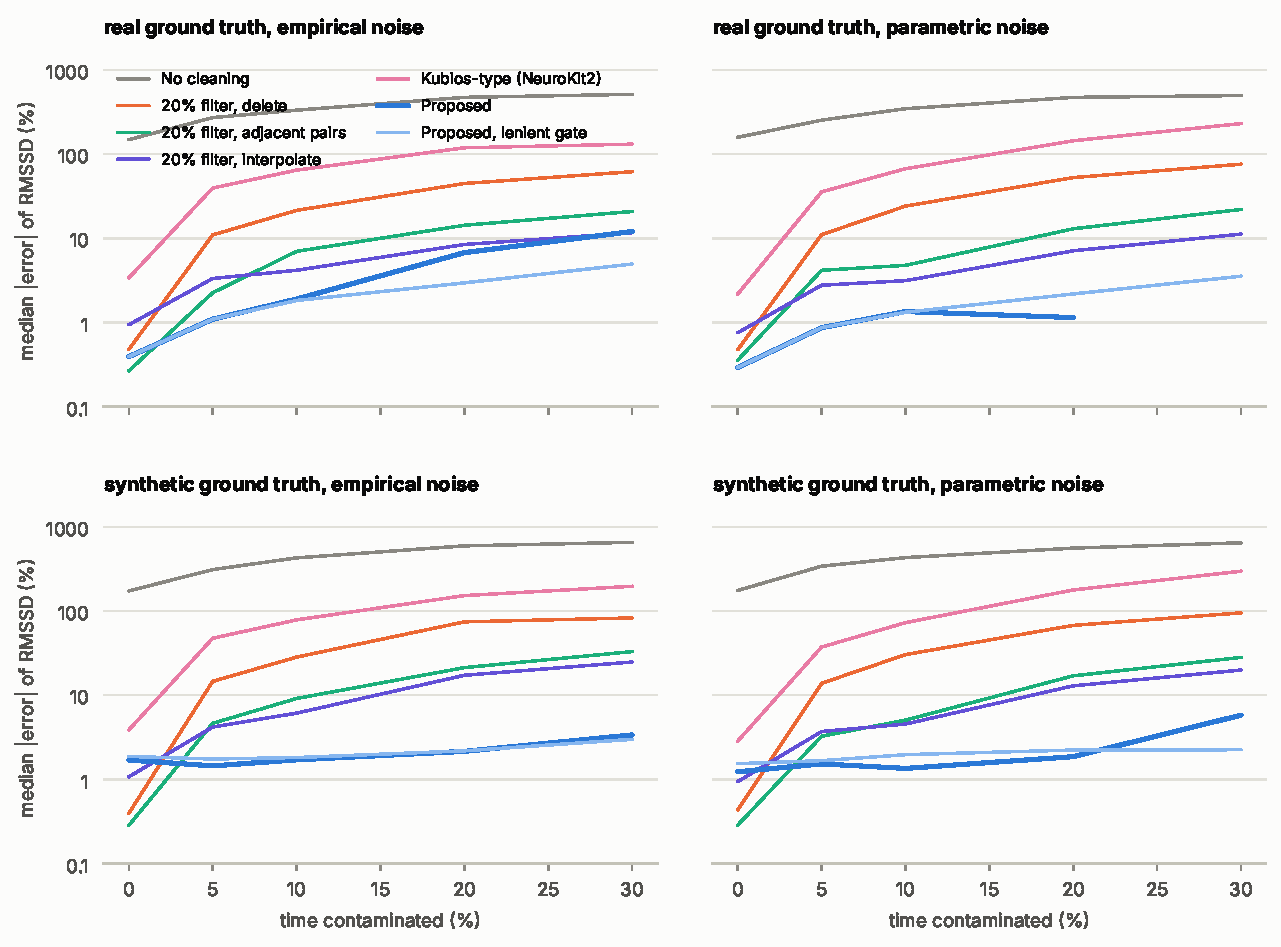
\includegraphics[width=0.92\linewidth]{figures/figS1_benchmark_grid.pdf}
\caption{Benchmark under every combination of ground truth and noise model.}
\end{figure}

\begin{figure}[H]
\centering
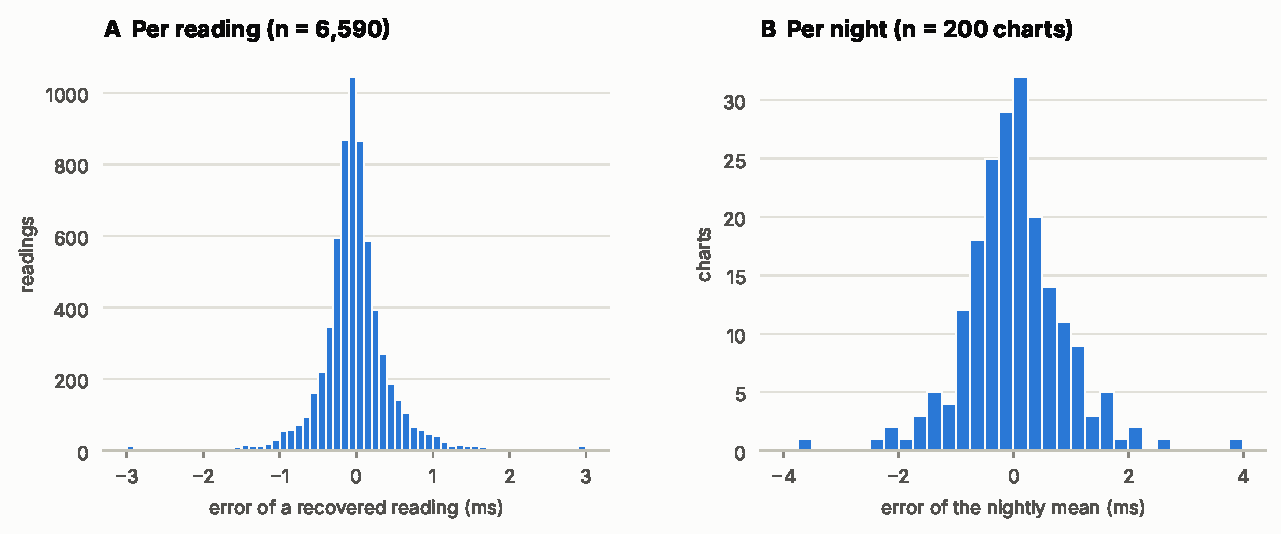
\includegraphics[width=0.92\linewidth]{figures/figS2_digitizer.pdf}
\caption{Digitiser validation on \nCharts{} synthetic nights: error of each recovered reading (A, n = \nDigReadings) and of the nightly mean (B).}
\end{figure}

\begin{figure}[H]
\centering
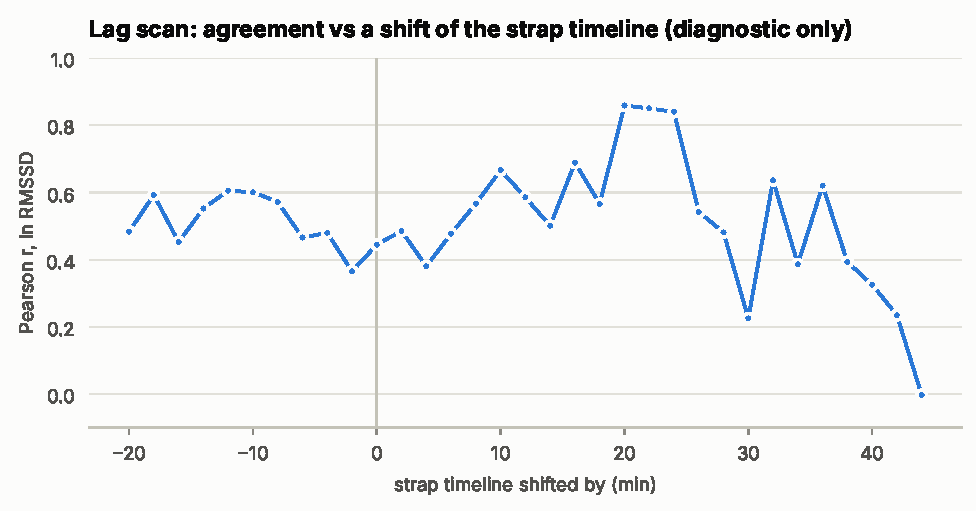
\includegraphics[width=0.7\linewidth]{figures/figS3_lag_scan.pdf}
\caption{Lag scan (diagnostic only): correlation between strap and watch ln RMSSD when the strap timeline (clock H1) is shifted.}
\end{figure}

\begin{figure}[H]
\centering
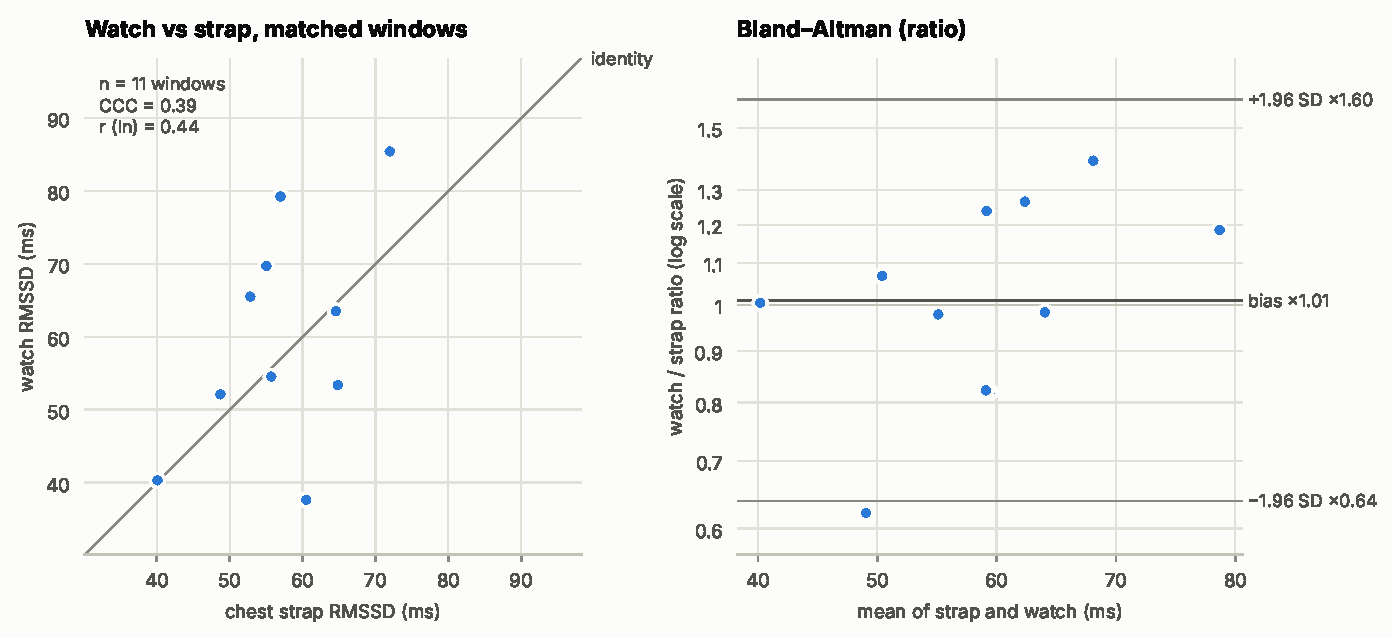
\includegraphics[width=0.92\linewidth]{figures/figS4_agreement.pdf}
\caption{Epoch-level agreement (clock H1, default gate): scatter with identity line and Bland--Altman plot on the ratio scale.}
\end{figure}

\begin{figure}[H]
\centering
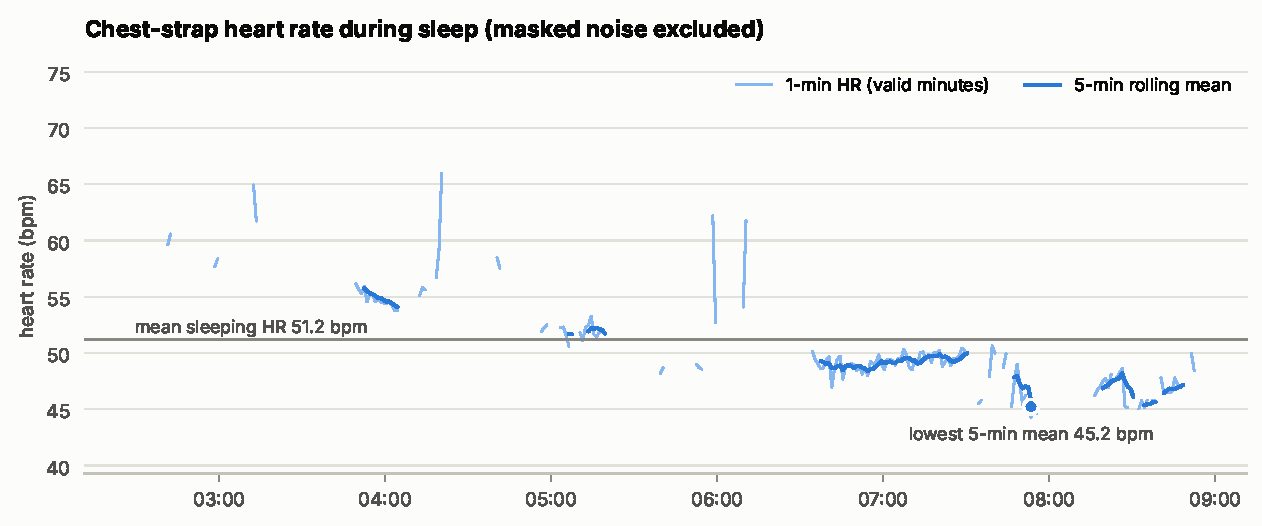
\includegraphics[width=0.92\linewidth]{figures/figS5_heart_rate.pdf}
\caption{Strap heart rate during sleep from usable beats (clock H1).}
\end{figure}

\end{document}
